\documentclass{article}
\usepackage{fullpage}
\usepackage{multicol,multirow}
\usepackage{tabularx}
\usepackage{ulem}
\usepackage[utf8]{inputenc}
\usepackage[russian]{babel}
\usepackage{pgfplots}
\usepackage{graphicx}

\begin{document}

\section*{Лабораторная работа №6 по курсу «Численные методы»}

Выполнил студент группы М8О-408Б-20 Попов Матвей.
\\
Преподаватель: Пивоваров Д.\,Е.

\subsection*{Цель}

Используя явную схему крест и неявную схему, решить начально-краевую задачу для 
дифференциального уравнения гиперболического типа. Аппроксимацию второго 
начального условия произвести с первым и со вторым порядком. Осуществить 
реализацию трех вариантов аппроксимации граничных условий, содержащих 
производные: двухточечная аппроксимация с первым порядком, трехточечная 
аппроксимация со вторым порядком, двухточечная аппроксимация со вторым 
порядком. В различные моменты времени вычислить погрешность численного решения 
путем сравнения результатов с приведенным в задании аналитическим решением 
$U(x, t)$. Исследовать зависимость погрешности от сеточных параметров $\tau$, 
$h$.

\subsection*{Вариант 1}
$$ \frac{\partial^2 u}{\partial t^2}=a^2 \frac{\partial^2u}{\partial x^2}, a > 0 $$
$$ u(0, t) = - \sin{(at)} $$
$$ u(\pi, t) = \sin{(at)} $$
$$ u(x, 0) = \sin{x} $$
$$ u(x, 0) = -a\cos{x} $$
Аналитическое решение: $$ U(x, t) = \sin{(x-at)} $$

\subsection*{О программе}
Модуль для вычислений написан на Go 1.21, модуль для визуализации написан 
на Python с использованием Jypiter Notebook. Реализации всех методов находятся 
в папке internal.

\subsection*{Инструкция к запуску}
Для запуска должны быть установлены Go 1.21 и Python 3, а также модули numpy и 
matplotlib. Для получения результатов и их визуализации достаточно запустить 
все ячейки в lab06.ipynb.

\subsection*{Результаты}
\begin{center}
Полученные вычисления на момент времени $ t = 0.5 $
\\
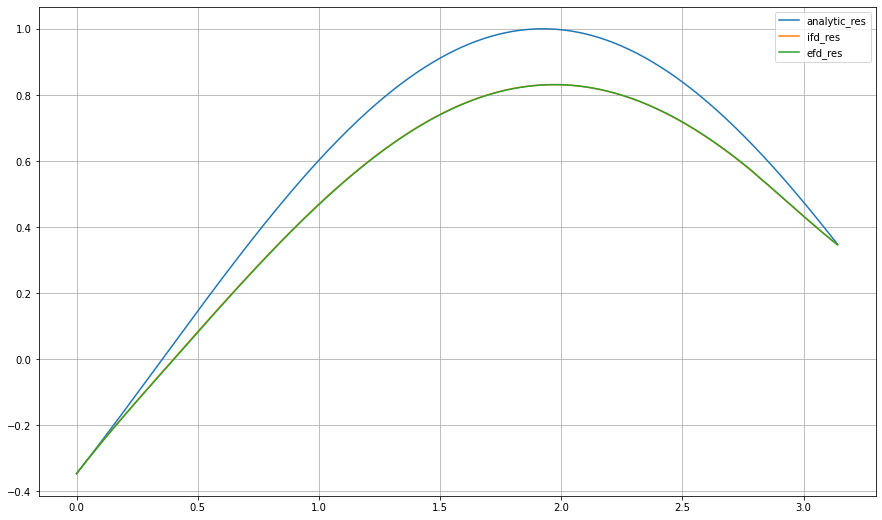
\includegraphics[scale=0.25]{img/img01.png}
\pagebreak
\\
Изменение погрешности
\\
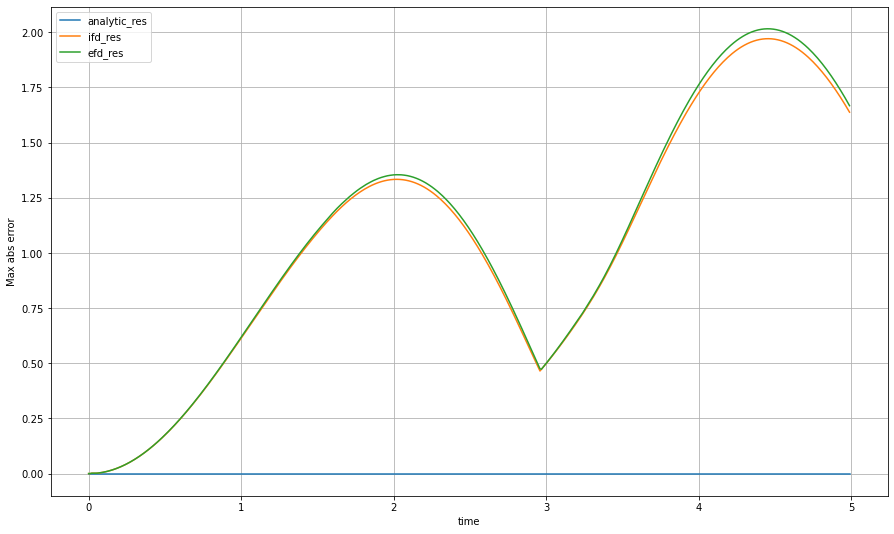
\includegraphics[scale=0.25]{img/img02.png}
\end{center}

\subsection*{Вывод}
Проделав лабораторную работу, я решил начально-краевую задачу для ДУ 
гиперболического типа двумя различными способами и проверил погрешности 
полученных вычислений.

\end{document}
